

%\addcontentsline{toc}{chapter}{Πειράματα}

\chapter{Πειράματα}
\par
Στην εργασία αυτή πραγματοποιήθηκε μια σειρά πειραμάτων τα οποία έχουν ως στόχο τόσο την διερεύνηση του αλγορίθμου ως προς την απόδοσή του σε εφαρμογές αναγνώρισης προτύπων όσο και στο πώς επιδρούν στο αποτέλεσμα του αλγορίθμου οι δύο παράμετροι που δέχεται σαν είσοδο. Οι παράμετροι αυτοί είναι ο αριθμός $k$ των κοντινών γειτόνων σύμφωνα με τους οποίους κατασκευάζεται ο πίνακας γειτνίασης του πρώτου βήματος του αλγορίθμου και η δεύτερη παράμετρος είναι ο αριθμός $d$ των τελικών διαστάσεων και οι οποίες καθορίζουν ουσιαστικά το αποτέλεσμα του τελευταίου βήματος. Ο σχεδιασμός των πειραμάτων έγινε με τρόπο ώστε να γίνει φανερό το πως επηρεάζουν την συμπεριφορά του αλγορίθμου οι παράμετροι αυτοί αλλά επίσης δόθηκε έμφαση στο να βρεθεί ο βέλτιστος συνδυασμός των δύο ανάλογα με το σετ δεδομένων κάθε πειράματος. 
\par
Eφαρμόζονται επίσης δύο τεχνικές με τις οποίες μπορεί κάποιος να αποφύγει το τεράστιο υπολογιστικό κόστος που απαιτείται. Συγκεκριμένα το τελευταίο βήμα του αλγορίθμου το οποίο είναι και το πιο απαιτητικό έχει πολυπλοκότητα $\mathcal{O}n^{3}$ στην γενική περίπτωση ενώ στην συγκεκριμένη περίπτωση λόγω του αραιού μητρώου $M$ είναι της τάξης $\mathcal{O}n^{2}$. Αντιλαμβανόμαστε λοιπόν ότι ακόμα και για ένα σχετικά μικρό σετ δεδομένων, για τα δεδομένα του κλάδου της μηχανικής μάθησης, το πρόβλημα που έχουμε να αντιμετωπίσουμε έχει απαγορευτικές διαστάσεις. 
\par
Ένα άλλο πρόβλημα που συναντάει κανείς κατά την εφαρμογή του αλγορίθμου σε κάποιο σετ δεδομένων είναι ο εξής περιορισμός. Ας υποθέσουμε ότι έχουμε ένα σύνολο δεδομένων μεγέθους $N$, απο τα οποία για κάποιον αριθμό $N1$ απο αυτά γνωρίζουμε την ετικέτα τους. Με τον όρο ετικέτα εννοούμε την τελική κλάση στην οποία ανήκει το κάθε δείγμα. Για τα υπόλοιπα δείγματα, έστω μεγέθους $N2$ δεν γνωρίζουμε την ετικέτα τους και είναι αυτά τα δείγματα για τα οποία θέλουμε να εξάγουμε το συμπέρασμα. Το συμπέρασμα αυτό είναι φυσικά η τελική απόφαση ως προς σε ποιά κλάση θα πρέπει να ταξινομηθεί το καθένα απο αυτά. Προφανώς η παραπάνω απόφαση προκύπτει λαμβάνοντας υπόψιν την πληροφορία την οποία μας δίνει το σύνολο των δεδομένων $N1$ τα οποία στον χώροτ της μηχανικής μάθησης αναφέρονται ως το σύνολο των δεδομένων εκπάιδευσης \textlatin{(train data)}. Τα υπόλοιπα δείγματα $N2$ αναφέρονται ως το σύνολο των δεδομένων αξιολόγησης \textlatin{(test data)}.
\par
Στο συγκεκριμένο λοιπόν έστω οτι τα δείγματα του αρχικού χώρου έχουν αρχική διάσταση μεγέθους $D$ και μέσω του αλγόριθμου μείωσης των διαστάσεων θέλουμε να βρεθούμε σε έναν νέο χώρο διάστασης $d$, προφανώς με $d < D$. Στην περίπτωση αυτή λοιπόν ο πιο απλός συλλογισμός που θα μπορούσε να κάνει κάποιος είναι να τρέξει τον αλγόριθμο \textlatin{LLE} πάνω στο σετ δεδομένων εκπαίδευσης ώστε να έχει ένα σύνολο δεδομένων μεγέθους $Ν1$, διάστασης $d$. Με τον ίδιο ακριβώς τρόπο θα μπορούσε να έχει και το δεύτερο σετ δεδομένων, τα δεδομένα αξιολόγησης, μεγέθους $N2$ και αυτά διάστασης $d$. Έπειτα για την ταξινόμηση των αποτελεσμάτων θα μπορούσε να εφαρμοστεί ο αλγόριθμος ταξινόμησης κοντινότερων γειτόνων ανάμεσα στο σετ αξιολόγησης με το σετ εκπαίδευσης. Έπειτα ανάλογα με την κλάση στην οποία ανήκει ο κοντινότερος γείτονας απο το σετ εκπαίδευσης για κάθε ένα στοιχείο των δεδομένων αξιολόγησης θα καταλήγαμε στην τελική απόφαση για την κλάση στην οποία ανήκει κάθε ένα απο τα δεδομένα του σετ $N2$. Προφανώς ο αλγόριθμος κοντινότερων γειτόνων θα εφασρμοστεί στον χώρο μειωμένης διάστασης μεγέθους $d$ χρησιμοποιώντας για παράδειγμα την μετρική της Ευκλείδιας απόστασης μεταξύ των σημείων.
\par
Αν λοιπόν εφαρμόσουμε την παραπάνω διαδικασία για κάποιο σετ δεδομένων, θα παρατηρήσουμε ότι το τελικό αποτέλεσμα της ταξινόμησής μας έχει πολύ μικρή επιτυχία. Αυτό συμβαίνει διότι, οι δύο υποχώροι οι οποίοι προέκυψαν απο το τελικό βήμα του αλγορίθμου \textlatin{LLE}, κατά το οποίο υπολογίστηκε ο νέος χώρος μειωμένης διάστασης για κάθε ένα απο τα δύο σύνολα δεδομένων, έχουν διαφορετική διανυσματική βάση και δεν μπορούν σε καμιά περίπτωση να συσχετιστούν μεταξύ τους ώστε να μπορέσουμε απο τα δεδομένα του ενός να καταλήξουμε σε κάποιο ορθό συμπέρασμα για τα δεδομένα του άλλου. Ο παραπάνω λοιπόν περιορισμός μας αναγκάζει να εφαρμόσουμε τον αλγόριθμο μείωσης των διαστάσεων στο σύνολο των δεδομένων, δηλαδή δίνοντας σαν είσοδο στον αλγόριθμο το σύνολο των δεδομένων μεγέθους $N = N1+N2$. Με τον τρόπο αυτό θα καταλήγαμε σε ένα νέο σετ δεδομένων μεγέθους $N$ αλλά διάστασης $d < D$. Τέλος σε αυτό το σετ δεδομένων τώρα μπορούμε κάλλιστα να εφαρμόσουμε τον αλγόριθμο εύρεσης κοντινότερων γειτόνων για κάθε ένα απο τα δεδομένα αξιολόγησης ως πρός τα δεδομένα εκπαίδευσης, φυσικά στον χώρο $d$ διστάσεων, και έτσι να καταλήξουμε στην ορθή ταξινόμηση των δειγμάτων $N2$ ως προς την κλάση στην οποία ανήκουν. 

\section{Μέθοδοι αντιμετώπισης της πολυπλοκότητας του προβλήματος}
\par
Όπως αντιλαμβανόμαστε απο την παραπάνω ανάλυση, η διαδικασία αυτή δεν είναι καθόλου πρακτική και μάλιστα δεν δίνει την δυνατότητα για λήψη αποφάσεων και ταξινόμησης δειγμάτων σε πραγματικό χρόνο. Αυτό διότι, για κάθε δείγμα αξιολόγησης που μας έρχεται ως είσοδος κάποια συγκεκριμένη χρονική στιγμή, και για το οποίο θέλουμε να καταλήξουμε σε κάποιο συμπέρασμα ως προς την κλάση στην οποία ανήκει, θα πρέπει να το ενσωματώνουμε στο σετ των δεδομένων εκπαίδευσης και στην συνέχεια να εκτελούμε τον αλγόριθμο \textlatin{LLE}. Αντιλαμβανόμαστε λοιπόν ότι η συγκεκριμένη διαδικασία δεν προσφέρεται σε καμιά περίπτωση για πρακτικές εφαρμογές κατα τις οποίες μάλιστα ο στόχος μας είναι να γίνει μείωση των διαστάσεων ώστε να μπορούμε να λαμβάνουμε ταχύτερα και ακριβέστερα αποτελέσματα. Το γεγονός αυτό μάλιστα αντιτίθεται στην συνολική φιλοσοφία της μείωσης των διαστάσεων κατά την οποία η μείωση των διαστάσεων μπορεί να επιταχύνει σε πολύ μεγάλο βαθμό τους απαραίτητους υπολογισμούς.

\subsection{Μέθοδος-1: Προβολή στον χώρο των δεδομένων εκπαίδευσης}
\par
Για τους λόγους λοιπόν οι οποίοι και αναφέρθηκαν παραπάνω, προκύπτει η ανάγκη να βρεθεί κάποιος τρόπος με τον οποίο να μπορούμε οποιαδήποτε στιγμή θέλουμε να ταξινομήσουμε κάποιο δεδομένο, χρησιμοποιώντας βέβαια την πληροφορία που μπορούν να μας δώσουν τα δεδομένα του σετ εκπαίδευσης. Την λύση στο πρόβλημα αυτό λοιπόν έρχεται να δώσει η λογική με την οποία λειτουργεί ο αλγόριθμος \textlatin{LLE}. Πιο συγκεκριμένα όπως αναφέραμε παραπάνω, η μέθοδος αυτή έχει ως στόχο να διατηρήσει τα γεωμετρικά τοπικά χαρακτηριστικά για κάθε ένα απο τα δείγματα του συνόλου εκπαίδευσης τόσο στον χώρο των αρχικών διαστάσεων όσο και στον τελικό χώρο μειωμένης διάστασης. Επίσης, λόγω του ότι η ενσωμάτωση των δεδομένων στον χώρο μειωμένης διάστασης γίνεται με τη χρήση του πίνακα βαρών $W$, ο οποίος προσδιορίζει για κάθε δείγμα του αρχικού χώρου την ανακατασκευή του μέσω των κοντινών του γειτόνων προκύπτει και η ιδέα της μεθόδου αυτής. Ο αντίστοιχος ψευδοκώδικας είναι ο παρακάτω
\selectlanguage{english}
\begin{algorithm}
   \caption{Projection Method}
    \begin{algorithmic}[1]   	
    	\State Let $Xtrain$ be $[D \times N1]$ Train\textunderscore dataset matrix and $Xtest$ be $[D \times N2]$ Test\textunderscore dataset matrix \Comment{N1,N2 declare the number of data and D the number of dimensions}
		\State 
    	
    	\State Let matrix $Y$ be $[d \times N1]$ Train data, after dimensionality reduction \Comment{ d < D}
    	\State
    	
    	\State Let matrix nn\textunderscore graph with size $[N1 \times N2]$ and all elements equal to zero
    	\State 
        
        \For{$i = 1$ to ${N_2}$}
            \State Find K-Nearest Neighbors from $Xtrain$
        \EndFor
        \State
		
		\State Keep the results to matrix IDX with size $[N2 \times K]$ \Comment{ K is the number of nearest neighbors}
		\For{$i = 1$ to ${N_2}$}
            \State Set IDX(i,1:K) cells of nn\textunderscore graph matrix equal to ones
            \State Make the matrix multiplication $Y \times$ nn\textunderscore graph$(1:N1,i)$ and store the result to $testY(1:d,i)$ \Comment{testY(:,i) is the result of dimensionality reduced $Xtest_i$}
        \EndFor
        \State 
        
        \State Final matrix testY has size $[d \times N2]$ and represents the projection of Xtest D-dimensional data into the d-dimensional emndedding subspace.  
        \State
        \State Now execute K-NN Classification between testY and Y datasets, to the d-dimensional space
	\end{algorithmic}
\end{algorithm}
\selectlanguage{greek}
\par
Απο την παραπάνω ανάλυση της μεθόδου γίνεται φανερό ότι μπορούμε να χρησιμοποιήσουμε την πληροφορία των δεδομένων Υ, τα οποία είναι τα δεδομένα εκπαίδευσης \textlatin{Xtrain} στον χώρο μειωμένης διάστασης, ώστε να ταξινομήσουμε οποιοδήποτε δείγμα απο το σετ δεδομένων αξιολόγησης. Το γεγονός αυτό, σε συνδυασμό με την ελάχιστη αύξηση του σφάλματος ταξινόμησης όπως θα γίνει φανερό στα αποτελέσματα των πειραμάτων κάνει την μέθοδο αυτή πολύ ελκυστική για πρακτικές εφαρμογές οι οποίες απαιτούν αποτελέσματα σε πραγματικό χρόνο και μάλιστα σε πολύ μεγάλες ταχύτητες γεγονός το οποίο εξασφαλίζεται απο τους υπολογισμούς στον χώρο των μειωμένωνδιαστάσεων $d$. Όπως μπορούμε να παρατηρήσουμε στο πρώτο βήμα της μεθόδου εφαρμόζουμε τον αλγόριθμο κοντινότερων γειτόνων στον χώρο των αρχικών διαστάσεων μεγέθους $D$, για το σετ δεδομένων αξιολόγησης ως προς το σετ δεδομένων εκπαίδευσης. Επομένων θα μπορούσαμε να ισχυριστούμε ότι το υπόλοιπο της διαδικασίας είναι περιττό εκτώς και αν το τελικό αποτέλεσμα ταξινόμησης είναι καλύτερο απο αυτό στον αρχικό χώρο. Παρ'όλα αυτά αν αναλογιστούμε ένα πολύ μεγάλο σετ δεδομένων με έναν αρκετά μεγάλο αριθμό διαστάσεων, όπως πρόκειται άλλωστε για τα περισσότερα πραγματικά σετ στον χώρο της αναγνώρισης προτύπων, τότε το γεγονός οτι απο το σημείο αυτό και μετά μπορούμε την πληροφορία των $D$ διαστάσεων να την πάρουμε απο τις πολύ λιγότερες όπως θα δούμε $d$ τελικές διαστάσεις αποτελεί τεράστιο κέρδος τόσο σε επόμενους υπολογισμούς όσο και στους όρους που απαιτούνται για την διαχείριση των δεδομένων.  
\par
Στην παραπάνω διαδικασία θεωρήσαμε ότι έχουμε ήδη εφαρμόσει τον αλγόριθμο \textlatin{LLE} στο σετ δεδομένων εκπαίδευσης και έτσι έχουμε το αποτέλεσμα, δηλαδή τα δεδομένα στον χώρο μειωμένης διάστασης στον πίνακα \textlatin{Y}. Το βήμα αυτό, παρ'ότι είναι σαφώς οικονομικότερο απο την περίπτωση στην οποία θα εφαρμόζαμε στον αλγόριθμο στο σύνολο των δεδομένων εκπαίδευσης αλλά και των δεδομένων αξιολόγησης, στις περισσότερες εφαρμογές απαιτεί πολύ μεγάλο μέγεθος μνήμης γεγονός που καθιστά τις περισσότερες φορές αδύνατη την εκτέλεση του αλγορίθμου. Για να διευκρινιστεί η διαδικασία εφαρμογής της μεθόδου αλλά και οι διαστάσεις των πινάκων κάθε βήματος δίνεται το παρακάτω διάγραμμα  
\newpage
\begin{figure}[t!]
\centering
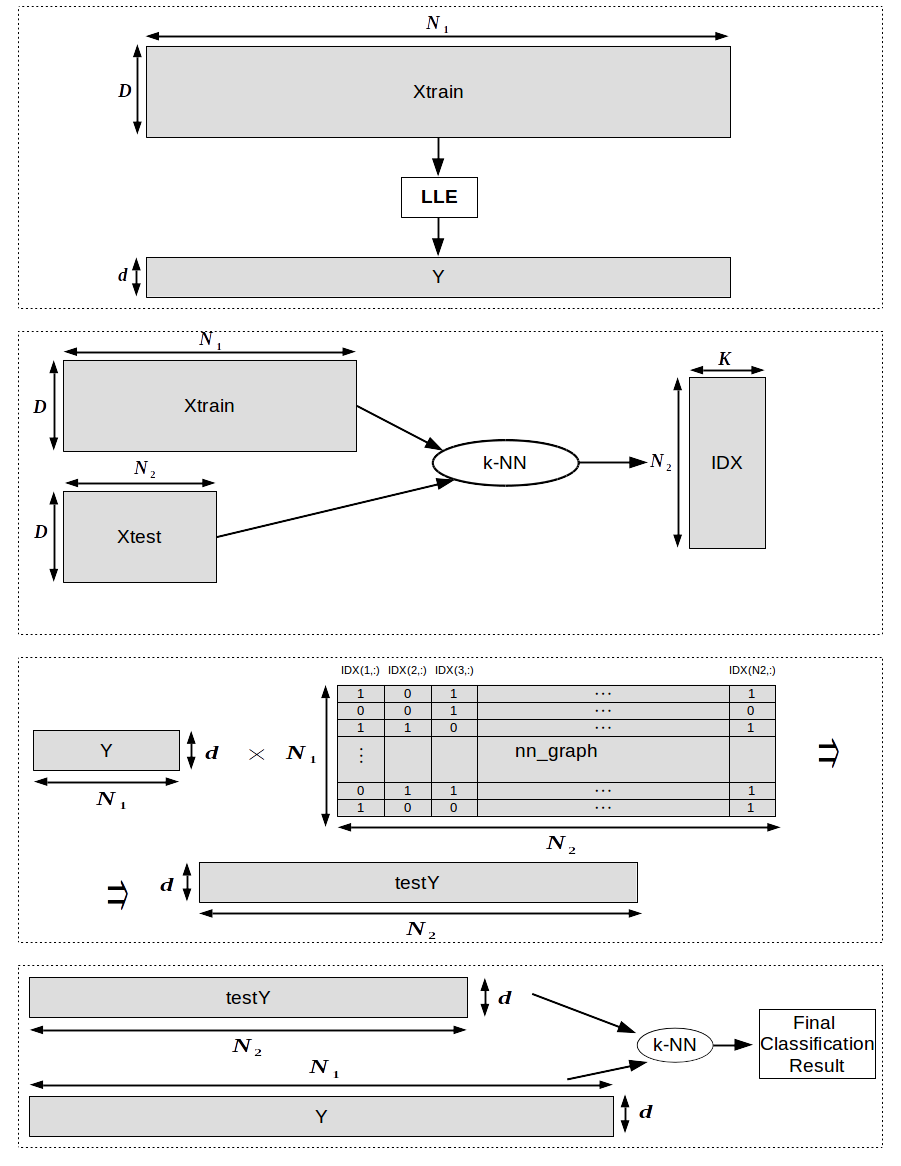
\includegraphics[scale=0.8]{figs/5.png}
\newline
\caption{ \textlatin{Method-1: Project test data, using adjacency matrix}.} 
\end{figure}
\newpage

\subsection{Μέθοδος-2: Δημιουργία υποχώρων και πλειοψηφική απόφαση ταξινόμησης }
\par
Για την αντιμετώπιση λοιπόν του παραπάνω προβλήματος μπορούμε να εφαρμόσουμε την Μέθοδο-2. Η βασική ιδέα της μεθόδου αυτής, όπως θα δούμε αναλυτικά και στον ψευδοκώδικα παρακάτω, είναι να διασπάσει το αρχικό σετ δεδομένων σε υποσύνολα απο τα οποία στην συνέχεια συνδυάζει την πληροφορία που δίνει το καθένα και εξάγει το τελικό αποτέλεσμα ταξινόμησης. Σημαντικό σημείο στην διαδικασία αυτή είναι η κατασκευή των υποσυνόλων να γίνει με τρόπο τέτοιο ώστε το καθένα απο αυτά να περιέχει την ίδια ποσότητα πληροφορίας, με την έννοια ότι θα πρέπει ο διαμοιρασμός των δειγμάτων κάθε κλάσης να γίνει ομοιόμορφα σε όλα τα υποσύνολα. Με τον τρόπο αυτό στην πραγματικότητα επιλύονται πολλά μικρά υποπροβλήματα όμοια με το αρχικό. Υποπροβλήματα δηλαδή τα οποία περιέχουν την ίδια πληροφορία με το αρχικό σετ δεδομένων εκπαίδευσης αλλά σε μικρότερη ποσότητα. Αν προσέξουμε ώστε το κάθε υποσύνολο να περιέχει αρκετά δείγματα ώστε να μπορέσει να διατηρηθεί το λείο της πολλαπλότητας το οποίο είναι απαίτηση του αλγορίθμου \textlatin{LLE} τότε το αποτέλεσμα της λύσης κάποιου υποχώρου θα είναι πολύ κοντά σε αυτό του αρχικού προβλήματος. Συνδυάζοντας την πληροφορία των υποχώρων στν συνέχεια, και καταλήγοντας στο αποτέλεσμα της ταξινόμησης ανάλογα με την πλειοψηφία των αποτελεσμάτων όλων των υποχώρων το κέρδος είναι διπλό. Μειώνεται καταρχήν δραματικό το κόστος υπολογισμού του αλγορίθμου \textlatin{LLE} λόγω της μείωσης κατά μεγάλο βαθμό των δειγμάτων στα οποία εφαρμόζεται. Επίσης με την διαδικασία του ψηφίσματος και της πλειοψηφικής τελικής επιλογής βελτιώνεται κατά πολύ το αποτέλεσμα της ταξινόμησης σε σχέση με αυτό του κάθε υποχώρου ξεχωριστά. 
\par
Για να γίνει κατανοητός ο τρόπος κατασκευής των υποσυνόλων αλλά και της συνολικής διαδικασίας της μεθόδου δίνεται ένα γράφημα το οποίο αναπαριστά τον διαμοιρασμό των δειγμάτων και έπειτα ο συνολικός ψευδοκώδικας τηε μεθόδου. Στο παρακάτω γράφημα έστω ότι το αρχικό μου σύνολο δεδομένων είναι το γνωστό σύνολο δεδομένων \href{http://yann.lecun.com/exdb/mnist/}{\textlatin{MNIST}} με μέγεθος έστω \textlatin{N} και το οποίο περιέχει δεδομένα τα οποία ανήκουν σε δέκα κλάσεις (ψηφία απο το 0 εως το 9). Επίσης κάθε εικόνα έχει γίνει μετατροπή σε ένα διάνυσμα-στήλη μεγέθους $[Width \times Height]$, έστω $D$. Έστω επίσης για το συγκεκριμένο παράδειγμα ότι επιλέγουμε να το χωρίσουμε σε 3 υποσύνολα. Η διαδικασία διαμοιρασμού των δειγμάτων φαίνεται γραφικά παρακάτω
\newpage
\begin{figure}[t!]
\centering
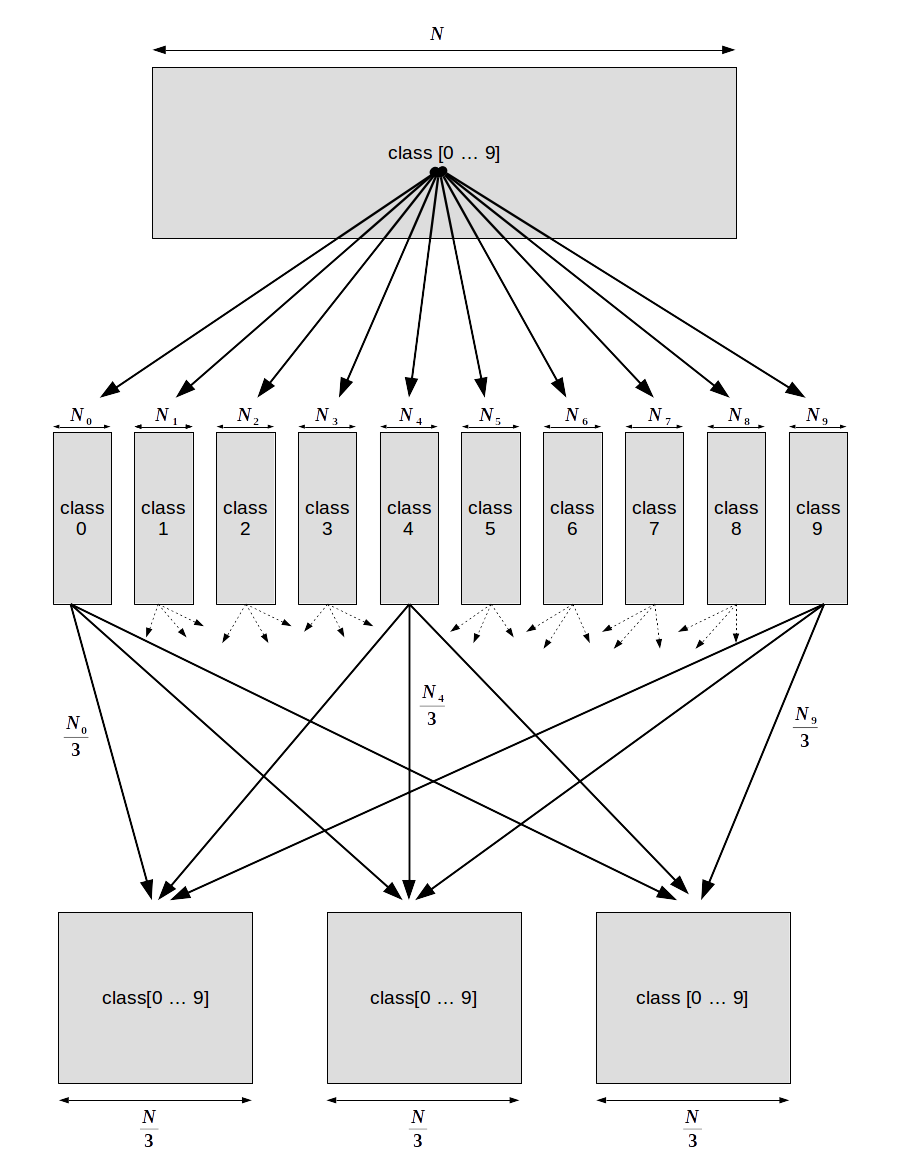
\includegraphics[scale=0.8]{figs/6.png}
\newline
\caption{ \textlatin{Split main dataset into sub-datasets}.} 
\end{figure}
\newpage
\par
Όπως φαίνεται αναλυτικά στο παραπάνω σχήμα το σύνολο των αρχικών κλάσεων ομαδοποιείται και στην συνέχεια μοιράζονται ανάλογα τα δείγματα κάθε κλάσης, ομοιόμορφα, σε όσα υποσύνολα έχουμε επιλέξει. Απο το σημείο αυτό λοιπόν μπορούμε πλέον να εφαρμόσουμε τον αλγόριθμο μέιωσης διστάσεων, \textlatin{LLE}, σε κάθε ένα απο τα τελικά υποσύνολα δεδομένων καταλήγοντας σε τρείς νέους χώρους μειωμένης προφανώς διάστασης. Να διευκρινιστεί στο σημείο αυτό ότι η διαδικασία προβολής των δεδομένων αξιολόγησης μπορεί να γίνει είτε ενσωματώνοντάς τα σε κάθε ένα απο τα τρία τελικά σετ δεδομένων πρίν την εφαρμογή του αλγορίθμου ή να εφαρμοστεί η Μέθοδος-1. Σύμφωνα με την Μέθοδο-1, όπως εξηγήσαμε και παραπάνω, θα γίνει μείωση των διαστάσεων για κάθε υποσύνολο και στην συνέχεια για κάθε ένα χωριστά θα γίνει η προβολή των δεδομένων αξιολόγησης στον χώρο μειωμένης διάστασης του καθενός. 
\par
Αφού εφαρμοστεί μια απο τις παραπάνω μεθόδους, ανεξαρτήτως ποια, μπορούμε πλέον για κάθε ένα σύνολο δεδομένων (τελικά σετ εκπαίδευσης ένα εως τρία και σετ αξιολόγησης στον χώρο μειωμένης διάστασης $d$) να εφαρμόσουμε τον αλγόριθμο κοντινότερων γειτόνων \textlatin{(k-NN)} και να κάνουμε την ταξινόμηση κάθε δείγματος του σετ αξιολόγησης, στην κλάση εκτίμησης για κάθε έναν απο τους τελικούς υποχώρους. Τέλος, πλειοψηφικά αποφασίζουμε σε ποιά κατηγορία ανήκει το κάθε δείγμα, λαμβάνοντας υπόψιν την ψήφο ως προς την κλάση ταξινόμησης του δείγματος απο τους τρείς υποχώρους. Με τον τρόπο αυτό, όπως θα φανεί και στα πειράματα παρακάτω, βελτιώνεται σε πολύ μεγάλο βαθμό το τελικό αποτέλεσμα της ταξινόμησης σε σχέση με αυτό των τριών υποχώρων. Η διαδικασία αυτή, παρουσιάζεται και γραφικά στο παρακάτω σχήμα
\newpage
\begin{figure}[t!]
\centering
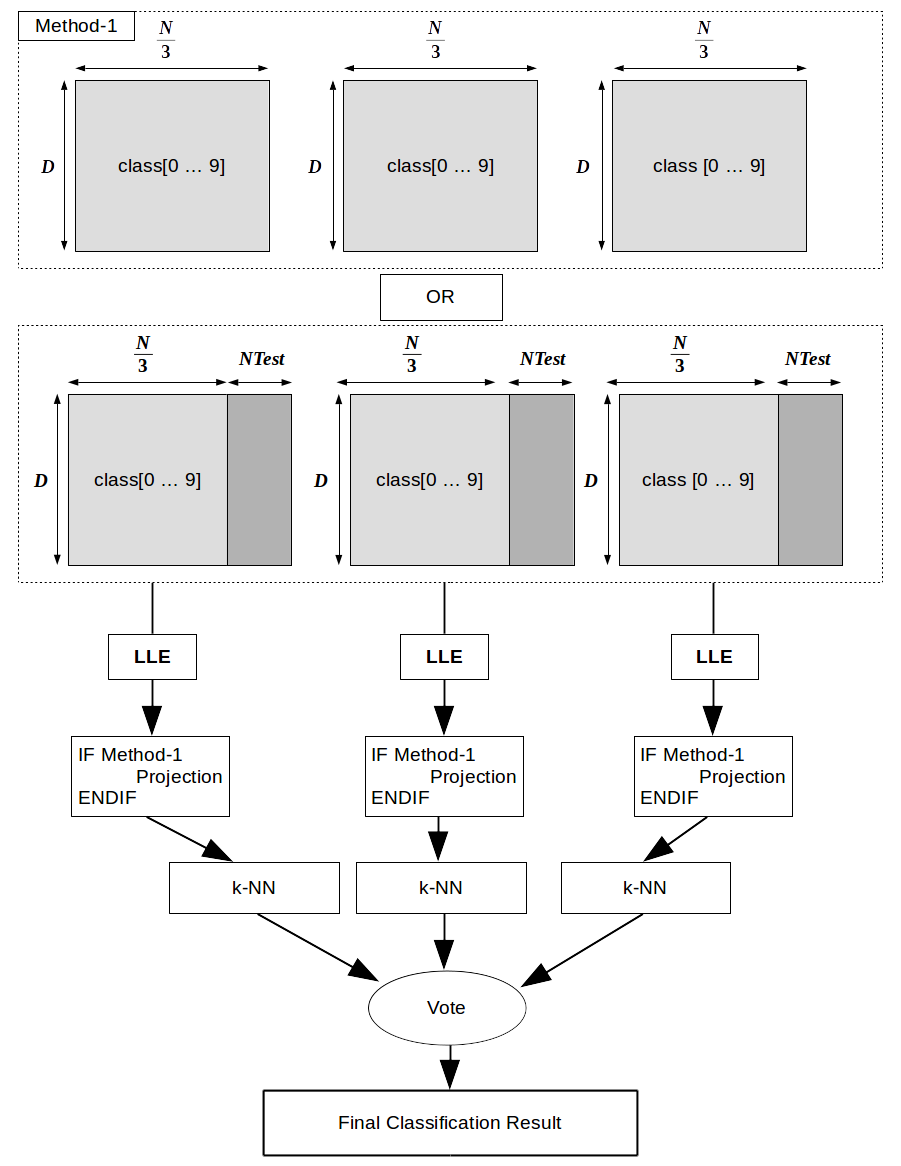
\includegraphics[scale=0.8]{figs/7.png}
\newline
\caption{ \textlatin{Sub datasets Dimensionality reduction and subspace classification voting}.} 
\end{figure}
\newpage

\section{Εφαρμογή του αλγορίθμου \textlatin{LLE} και των μεθόδων σε πραγματικά σετ δεδομένων}
\par
Στην εργασία αυτή δόθηκε έμφαση στην μελέτη του αλγορίθμου σε συγκεκριμένα σετ δεδομένα αλλά παράλληλα διερευνήθηκε σε μεγάλο βαθμό το πως επηρεάζουν την συμπεριφορά του οι παράμετροι που δέχεται ως είσοδο απο τον χρήστη. Αυτές είναι ο αριθμός των κοντινότερων γειτόνων \textlatin{(K)} για το πρώτο βήμα του αλγορίθμου και ο αριθμός των τελικών διστάσεων \textlatin{(d)} για το τελικό βήμα του. Επίσης, γίνεται σύγκριση στην απόδοση του αλγορίθμου ταξινόμησης κοντινότερων γειτόνων \textlatin{(k-NN)} για τον χώρο αρχικών διαστάσεων \textlatin{D} και αυτού των τελικών \textlatin{d}. 

\subsection{Πειράματα και Αποτελέσματα}
\par
\href{http://yann.lecun.com/exdb/mnist/}{\textbf{\textlatin{MNIST: }}}Το πρώτο σετ δεδομένων το οποίο χρησιμοποιήθηκε είναι το πολύ γνωστό και ευρέως χρησιμοποιούμενο σετ δεδομένων στον χώρο της αναγνώρισης προτύπων, \href{http://yann.lecun.com/exdb/mnist/}{\textlatin{MNIST}}. Το σετ αυτό αποτελείται απο 70.000 εικόνες, διάστασης $[28 \times 28]$ \textlatin{pixel}, οι οποίες περιέχουν χειρόγραφα ψηφία. Οι 60.000 απο αυτές ανήκουν στο σετ εκπαίδευσης και οι 10.000 στο σετ αξιολόγησης. Για την είσοδο των δεδομένων στον αλγόριθμο, εφαρμόστηκε η λεξικογραφική διάταξη σε κάθε μια απο τις εικόνες, καταλήγοντας σε ένα διάνυσμα διάστασης $D = 784$. Τέλος, να διευκρινιστεί ότι το τελικό αποτέλεσμα ταξινόμησης, για τα σετ δεδομένων με τα ψηφία είναι το μέσο σφάλμα ταξινόμησης δηλαδή το άθροισμα του σφάλματος κάθε κλάσης προς τον συνολικό αριθμό των κλάσεων. Η επιλογή αυτή έγινε, διότι η μετρική αυτή δίνει έναν πολύ πιο ακριβές και γενικευμένο αποτέλεσμα ως προς την απόδοση του αλγορίθμου.
 
\subsubsection{Πειράματα - \textlatin{MNIST}}
\par
Στο πρώτο πείραμα με αυτό το σετ δεδομένων διερευνήθηκε αρχικά η συμπεριφορά του αλγορίθμου ως προς την απόδοση του αποτελέσματος ταξινόμησης μετά την μείωση των διαστάσεων. Οι παράμετροι οι οποίες αξιολογήθηκαν είναι ο αριθμός Κ των κοντινότερων γειτόνων, ο αριθμός των τελικών διαστάσεων \textlatin{d} αλλά και ο αριθμός των υποσυνόλων της Μεθόδου-2. Συγκεκριμένα για τον αριθμό κοντινότερων γειτόνων του πρώτου βήματος του αλγορίθμου δόθηκαν οι τιμές $K = 6,7,8,9,10,12,16,20,24,32,64$, για τον αριθμό των τελικών διαστάσεων του τελευταίου βήματος οι τιμές $d = 10,16,20,24,32,40,52,64,96,128,256$ και για τον αριθμό των δειγμάτων των υποσυνόλων οι τιμές $batch\textunderscore size = 10.000,20.000,60.000$ .Δηλαδή χωρίσαμε το σετ δεδομένων εκπαίδευσης των 60.000 εικόνων σε 6,3,1 υποσύνολα αντίστοιχα. Για το πείραμα αυτό δεν χρησιμοποιήσαμε την μέθοδο-1, δηλαδή σε κάθε υποσύνολο κάθε φορά ενσωματώσαμε τα δεδομένα αξιολόγησης στα δεδομένα εκπαίδευσης και στην συνέχεια εφαρμόσαμε τον αλγόριθμο για την μείωση των διαστάσεων στο σύνολο των δεδομένων αυτών. Για την εξαγωγή του τελικού αποτελέσματος εφαρμόστηκε ο αλγόριθμος \textlatin{k-NN} με $k=2$. Το μικρότερο ποσοστό σφάλματος ταξινόμησης δόθηκε για τις παραμέτρους $K=12, d=128, batch\textunderscore size=60.000$, με τιμή 3.06\% έναντι του 3.5\% το οποίο είναι το σφάλμα ταξινόμησης στον χώρο των αρχικών διαστάσεων \textlatin{D}. Πολύ μεγάλο ενδιαφέρον παρουσιάζει το γεγονός ότι το σφάλμα για τις παραμέτρους $K=8, d=10, batch\textunderscore size=60.000$ ισούτε με 3.31\% το οποίο είναι και αυτό μικρότερο απο την ταξινόμηση πρίν την μείωση διαστάσεων. Αξίζει να δοθεί έμφαση στην συγκεκριμένη αυτή περίπτωση διότι έχουμε καλύτερο ποσοστό ταξινόμησης έπειτα απο δραματική μείωση των διαστάσεων, αφού απο τις 784 αρχικές επιλέγουμε τελικά να κρατήσουμε 10 τελικές. 
\par
Παρατηρώντας τα αποτελέσματα των παρακάτω πινάκων μπορεί να παρατηρήσει κανείς ότι για την περίπτωση όπου έχουμε 64 ή περισσότερες τελικές διαστάσεις το τελικό ποσοστό σφάλατος είναι μικρότερο ή οριακά ίσο με αυτό του χώρου των αρχικών διαστάσεων. Το ίδιο ισχύει και για την περίπτωση στην οποία έχουμε $batch_size=20.000$. Το γεγονός αυτό μας δίνει ένα πολύ μεγάλο πλεονέκτημα διότι χωρίζοντας το σετ δεδομένων εκπαίδευσης των 60.000 δειγμάτων, σε 3 υποσύνολα έχουμε τεράστια μείωση στο κόστος των υπολογισμών αλλά και στην διαθέσιμη μνήμη η οποία απαιτείται για την εκτέλεση του αλγορίθμου. Ακόμα πιο ενδιαφέρον είναι το αποτέλεσμα του πειράματος με παραμέτρους $K=10, d=128, batch\textunderscore size=10.000$ για το οποίο έχουμε σφάλμα ταξινόμησης 3.31\%, αποτέλεσμα μικρότερο απο αυτό των αρχικών διαστάσεων και μάλιστα πολύ οικονομικότερο στον χρόνο υπολογισμού διότι στην περίπτωση αυτή έχουμε χωρίσει το σετ εκπαίδευσης σε 6 μικρούς σχετικά υποχώρους οι οποίοι μειώνουν την πολυπλοκότητα επίλυσης του προβλήματος κατά πολλές τάξεις μεγέθους. Οι παρακάτω πίνακες δείχνουν τα αποτέλεσμα του σφάλματος ταξινόμησης για όλους τους συνδυασμούς των παραμέτρων, και φανερώνουν σημαντικά στοιχεία για την αποτελεσματικότητα της μείωσης των διαστάσεων.

\selectlanguage{english}
\begin{table}[H]
\centering
\label{tab:table1}
\begin{tabular}{|c|c|c|c|c|c|c|c|c|c|c|c|}
\hline
& K=6 & K=7 & K=8 & K=9 & K=10 & K=12 & K=16 & K=20 & K=24 & K=32 & K=64 \\
\hline
d=10 & 4.07 & 4.18 & 4.20 & 4.48 & 4.60 & 4.69 & 5.82 & 7.35 & 9.87 & 13.2 & 22.83 \\
d=16 & 3.91 & 3.98 & 4.06 & 4.22 & 4.20 & 4.36 & 5.29 & 5.92 & 7.81 & 10.45 & 17.10 \\
d=20 & 4.03 & 3.99 & 4.16 & 4.15 & 4.14 & 4.44 & 4.96 & 5.69 & 6.95 & 9.31 & 15.55 \\
d=24 & 4.13 & 4.05 & 4.10 & 4.14 & 4.22 & 4.13 & 4.77 & 5.40 & 6.35 & 8.32 & 14.12 \\
d=32 & 3.92 & 3.91 & 4.03 & 3.98 & 4.07 & 4.18 & 4.27 & 5.07 & 5.78 & 7.37 & 12.36 \\
d=40 & 4.00 & 3.82 & 3.90 & 3.99 & 3.97 & 4.03 & 4.15 & 4.72 & 5.22 & 6.41 & 11.93 \\
d=52 & 3.93 & 3.78 & 3.97 & 3.83 & 3.93 & 3.97 & 4.17 & 4.37 & 4.89 & 6.30 & 10.74 \\
d=64 & 3.95 & 3.76 & 3.77 & 3.87 & 3.80 & 3.87 & 3.81 & 4.14 & 4.61 & 6.05 & 10.28 \\
d=96 & 4.02 & 3.6 & 3.7 & 3.68 & 3.68 & 3.72 & 3.63 & 3.90 & 4.22 & 5.51 & 10.06 \\
d=128 & 3.89 & 3.67 & 3.59 & 3.51 & 3.31 & 3.66 & 3.60 & 3.98 & 4.43 & 5.29 & 10.01 \\
d=256 & 3.77 & 3.64 & 3.51 & 3.33 & 3.47 & 3.34 & 3.56 & 4.06 & 4.61 & 5.40 & 9.43 \\
\hline
\end{tabular}
\caption{MNIST k-NN Classification Mean Average (\%) Error (Method-2: subspaces=6)}
\end{table}

\begin{table}[H]
\centering
\label{tab:table2}
\begin{tabular}{|c|c|c|c|c|c|c|c|c|c|c|c|}
\hline
& K=6 & K=7 & K=8 & K=9 & K=10 & K=12 & K=16 & K=20 & K=24 & K=32 & K=64 \\
\hline
d=10 & 3.90 & 3.75 & 3.92 & 4.07 & 3.97 & 4.60 & 5.49 & 6.64 & 10.66 & 14.99 & 31.58 \\
d=16 & 3.88 & 3.80 & 3.75 & 4.00 & 3.87 & 4.19 & 4.86 & 5.63 & 7.55 & 10.45 & 20.65 \\
d=20 & 3.81 & 3.82 & 3.84 & 3.89 & 3.95 & 4.01 & 4.61 & 5.40 & 6.92 & 9.88 & 17.65 \\
d=24 & 3.73 & 3.73 & 3.81 & 3.87 & 3.87 & 3.90 & 4.47 & 5.29 & 6.19 & 9.28 & 15.88 \\
d=32 & 3.78 & 3.63 & 3.72 & 3.65 & 3.82 & 3.79 & 4.26 & 4.94 & 5.53 & 8.23 & 13.69 \\
d=40 & 3.73 & 3.70 & 3.73 & 3.71 & 3.71 & 3.75 & 4.09 & 4.51 & 5.57 & 6.90 & 12.43 \\
d=52 & 3.77 & 3.73 & 3.61 & 3.66 & 3.61 & 3.68 & 4.05 & 4.30 & 4.85 & 6.36 & 11.09 \\
d=64 & 3.73 & 3.65 & 3.66 & 3.57 & 3.52 & 3.76 & 3.81 & 4.21 & 4.79 & 5.91 & 10.56 \\
d=96 & 3.65 & 3.64 & 3.51 & 3.56 & 3.49 & 3.41 & 3.63 & 3.92 & 4.23 & 5.25 & 10.02 \\
d=128 & 3.81 & 3.53 & 3.52 & 3.48 & 3.47 & 3.35 & 3.71 & 3.88 & 4.22 & 5.21 & 9.48 \\
d=256 & 3.57 & 3.46 & 3.39 & 3.30 & 3.25 & 3.37 & 3.27 & 3.66 & 4.32 & 5.47 & 8.73 \\
\hline
\end{tabular}
\caption{MNIST k-NN Classification Mean Average (\%) Error (Method-2: subspaces=3)}
\end{table}

\begin{table}[H]
\centering
\label{tab:table3}
\begin{tabular}{|c|c|c|c|c|c|c|c|c|c|c|c|}
\hline
& K=6 & K=7 & K=8 & K=9 & K=10 & K=12 & K=16 & K=20 & K=24 & K=32 & K=64 \\
\hline
d=10 & 3.56 & 3.35 & 3.31 & 3.53 & 3.63 & 4.10 & 4.48 & 5.59 & 9.41 & 16.72 & 37.48 \\
d=16 & 3.48 & 3.35 & 3.44 & 3.42 & 3.40 & 3.67 & 4.10 & 5.00 & 7.07 & 11.39 & 25.14 \\
d=20 & 3.41 & 3.31 & 3.40 & 3.40 & 3.41 & 3.53 & 4.08 & 4.56 & 6.57 & 9.63 & 22.04 \\
d=32 & 3.45 & 3.39 & 3.42 & 3.51 & 3.35 & 3.30 & 3.90 & 4.55 & 6.18 & 9.35 & 19.53 \\
d=24 & 3.62 & 3.33 & 3.47 & 3.45 & 3.26 & 3.40 & 3.51 & 4.24 & 5.36 & 8.45 & 16.59 \\
d=40 & 3.52 & 3.34 & 3.54 & 3.46 & 3.37 & 3.37 & 3.48 & 4.18 & 5.14 & 7.91 & 14.58 \\
d=52 & 3.43 & 3.13 & 3.41 & 3.34 & 3.35 & 3.44 & 3.44 & 3.64 & 4.96 & 7.15 & 12.27 \\
d=64 & 3.52 & 3.20 & 3.36 & 3.35 & 3.34 & 3.43 & 3.46 & 3.68 & 4.89 & 6.52 & 11.06 \\
d=96 & 3.24 & 3.10 & 3.26 & 3.21 & 3.22 & 3.33 & 3.35 & 3.61 & 4.34 & 6.05 & 10.37 \\
d=128 & 3.19 & 3.25 & 3.11 & 3.30 & 3.12 & 3.06 & 3.34 & 3.55 & 4.06 & 5.84 & 10.18 \\
d=256 & 3.18 & 3.34 & 3.22 & 3.21 & 3.18 & 3.14 & 3.17 & 3.62 & 3.88 & 5.72 & 9.51 \\
\hline
\end{tabular}
\caption{MNIST k-NN Classification Mean Average (\%) Error (No subspaces)}
\end{table}

\selectlanguage{greek}
\par
Απο την στιγμή που απο τα παραπάνω αποτελέσματα επιβεβαιώθηκε το γεγονός ότι μπορούμε να πάρουμε καλύτερο αποτέλεσμα ταξινόμησης εφαρμόζοντας την μέθοδο της διάσπασης του σετ εκπαίδευσης σε υποσύνολα, και μάλιστα με την διαδικασία της ταξινόμησης να είναι πολυ οικονομικότερη αλλά και γρηγορότερη, εστιάσαμε στον τρόπο με τον οποίο γίνεται η επιλογή των δεδομένων με σκοπό την δημιουργία των τελικών υποσυνόλων. Σκεφτήκαμε λοιπόν την περίπτωση για την οποία θα μπορούσε να δημιουργηθεί ένας υποχώρος, ο οποίος να περιέχει την χρήσιμη πληροφορία απο ολόκληρο το σετ εκπαίδευσης. Δηλαδή, σύμφωνα με την παραπάνω μέθοδο απο όλα τα τελικά υποσύνολα. Ο τρόπος με τον οποίο προσπαθήσαμε να οδηγηθούμε σε αυτό το αποτέλεσμα είναι η εφαρμογή αλγορίθμων ομαδοποίησης των δεδομένων. Συγκεκριμένα εφαρμόστηκε ο αλγόριθμος \href{https://en.wikipedia.org/wiki/K-means_clustering}{\textlatin{K-means}} επιλέγοντας σαν τελικά αντιπροσωπευτικά σημεία για το τελικό σύνολο δεδομένων εκπαίδευσης, το αποτέλεσμα του αλγορίθμου το οποίο είναι τα κεντροειδή σημεία τα οποία αντιπροσωπεύουν τις επιμέρους ομάδες. Δοκιμάστηκαν διαφορετικές τιμές για το σύνολο των τελικών κεντροειδών, καταλήγοντας στο βέλτιστο αποτέλεσμα για την περίπτωση στην οποία έχουμε $K=9, d=128, clustSize=20.000$. Το σφάλμα της ταξινόμησης για την περίπτωση αυτή είναι 3.28\%, μικρότερο απο αυτό των αρχικών διαστάσεων (3.5\%). Συγκεκριμένες τιμές για τις παραμέτρους είναι $K=8,9,10,12,16,20$, \textlatin{d} όπως και στο προηγούμενο ερώτημα και $clustSize=5.000, 10.000, 15.000, 20.000$. Το σύνολο των αποτελεσμάτων φαίνεται στους παρακάτω πίνακες
\selectlanguage{english}
\begin{table}[H]
\centering
\label{tab:table4}
\begin{tabular}{|c|c|c|c|c|c|c|}
\hline
& K=8 & K=9 & K=10 & K=12 & K=16 & K=20 \\
\hline
d=10 & 5.91 & 6.75 & 7.28 & 8.78 & 10.35 & 16.21 \\
d=16 & 5.31 & 6.15 & 6.44 & 7.54 & 9.25 & 11.56 \\
d=20 & 5.16 & 5.25 & 5.31 & 6.37 & 8.66 & 10.85 \\
d=24 & 5.11 & 5.08 & 5.13 & 6.09 & 7.97 & 10.13 \\
d=32 & 5.01 & 5.10 & 5.18 & 5.86 & 6.75 & 9.18 \\
d=40 & 4.90 & 5.00 & 4.81 & 5.35 & 6.50 & 8.32 \\
d=52 & 5.08 & 5.02 & 5.00 & 5.53 & 6.48 & 7.51 \\
d=64 & 4.90 & 4.99 & 5.02 & 5.61 & 6.08 & 6.97 \\
d=96 & 4.76 & 4.82 & 5.05 & 5.29 & 5.87 & 6.42 \\
d=128 & 4.79 & 4.96 & 5.02 & 5.22 & 5.70 & 5.77 \\
d=164 & 4.88 & 4.98 & 4.97 & 5.38 & 5.41 & 5.47 \\
d=196 & 5.08 & 5.09 & 5.11 & 5.42 & 5.39 & 5.32 \\
d=256 & 5.33 & 5.33 & 5.30 & 5.17 & 5.45 & 5.18 \\
\hline
\end{tabular}
\caption{MNIST k-NN Classification Mean Average (\%) Error (K-means subsampling - 5.000 centroids)}
\end{table}

\begin{table}[H]
\centering
\label{tab:table5}
\begin{tabular}{|c|c|c|c|c|c|c|}
\hline
& K=8 & K=9 & K=10 & K=12 & K=16 & K=20 \\
\hline
d=10 & 4.98 & 5.87 & 6.18 & 7.32 & 9.04 & 13.17 \\
d=16 & 4.69 & 4.89 & 5.03 & 6.49 & 7.66 & 11.22 \\
d=20 & 4.37 & 4.70 & 4.83 & 5.88 & 6.82 & 9.74 \\
d=24 & 4.33 & 4.62 & 4.67 & 5.49 & 6.50 & 8.30 \\
d=32 & 4.38 & 4.53 & 4.72 & 5.20 & 6.08 & 7.55 \\
d=40 & 4.35 & 4.35 & 4.87 & 5.13 & 5.76 & 6.70 \\
d=52 & 4.31 & 4.18 & 4.52 & 5.26 & 5.78 & 6.61 \\
d=64 & 4.31 & 4.42 & 4.60 & 5.06 & 5.43 & 6.44 \\
d=96 & 4.13 & 4.23 & 4.30 & 4.88 & 5.14 & 5.67 \\
d=128 & 4.07 & 4.06 & 4.32 & 4.68 & 5.01 & 5.64 \\
d=164 & 3.98 & 4.13 & 4.37 & 4.67 & 5.08 & 5.09 \\
d=196 & 4.19 & 4.38 & 4.39 & 4.65 & 4.85 & 5.17 \\
d=256 & 4.37 & 4.48 & 4.54 & 4.65 & 4.90 & 4.82 \\
\hline
\end{tabular}
\caption{MNIST k-NN Classification Mean Average (\%) Error (K-means subsampling - 10.000 centroids)}
\end{table}

\begin{table}[H]
\centering
\label{tab:table6}
\begin{tabular}{|c|c|c|c|c|c|c|}
\hline
& K=8 & K=9 & K=10 & K=12 & K=16 & K=20 \\
\hline
d=10 & 4.61 & 4.86 & 5.54 & 6.35 & 8.23 & 12.80 \\
d=16 & 4.09 & 4.27 & 4.72 & 5.18 & 7.38 & 9.52 \\
d=20 & 3.94 & 4.21 & 4.47 & 5.12 & 6.91 & 8.38 \\
d=24 & 3.87 & 4.05 & 4.39 & 4.86 & 6.48 & 7.91 \\
d=32 & 4.05 & 4.07 & 4.22 & 4.65 & 5.32 & 7.49 \\
d=40 & 3.72 & 3.88 & 4.11 & 4.43 & 4.94 & 6.75 \\
d=52 & 3.78 & 3.97 & 4.00 & 4.30 & 4.74 & 6.2 \\
d=64 & 3.79 & 3.94 & 4.07 & 4.38 & 4.73 & 5.81 \\
d=96 & 3.76 & 3.81 & 4.14 & 4.50 & 4.64 & 5.45 \\
d=128 & 3.74 & 3.96 & 4.25 & 4.34 & 4.67 & 5.08 \\
d=164 & 3.96 & 4.18 & 4.08 & 4.39 & 4.76 & 4.69 \\
d=196 & 4.03 & 4.18 & 4.04 & 4.30 & 4.73 & 4.72 \\
d=256 & 3.98 & 4.18 & 4.04 & 4.42 & 4.93 & 4.52 \\
\hline
\end{tabular}
\caption{MNIST k-NN Classification Mean Average (\%) Error (K-means subsampling - 15.000 centroids)}
\end{table}

\begin{table}[H]
\centering
\label{tab:table7}
\begin{tabular}{|c|c|c|c|c|c|c|}
\hline
& K=8 & K=9 & K=10 & K=12 & K=16 & K=20 \\
\hline
d=10 & 4.29 & 4.52 & 4.83 & 5.65 & 6.97 & 10.78 \\
d=16 & 3.82 & 4.10 & 4.18 & 4.99 & 6.01 & 7.69 \\
d=20 & 3.80 & 4.00 & 4.02 & 4.70 & 5.59 & 7.58 \\
d=24 & 3.82 & 3.96 & 4.03 & 4.45 & 5.01 & 6.78 \\
d=32 & 3.91 & 3.92 & 4.14 & 4.34 & 4.62 & 6.02 \\
d=40 & 3.74 & 3.75 & 4.03 & 4.42 & 4.57 & 5.67 \\
d=52 & 3.73 & 3.64 & 3.88 & 4.23 & 4.54 & 5.21 \\
d=64 & 3.69 & 3.58 & 3.83 & 4.17 & 4.30 & 5.01 \\
d=96 & 3.54 & 3.60 & 3.58 & 3.92 & 4.31 & 4.85 \\
d=128 & 3.42 & 3.28 & 3.53 & 3.88 & 4.18 & 4.88 \\
d=164 & 3.44 & 3.32 & 3.41 & 3.79 & 4.57 & 4.74 \\
d=196 & 3.31 & 3.40 & 3.55 & 3.74 & 4.39 & 4.62 \\
d=256 & 3.60 & 3.47 & 3.58 & 3.71 & 4.20 & 4.43 \\
\hline
\end{tabular}
\caption{MNIST k-NN Classification Mean Average (\%) Error (K-means subsampling - 20.000 centroids)}
\end{table}

\selectlanguage{greek}
\par
Στον παραπάνω πίνακα ενδιαφέρον παρουσιάζει το γεγονός ότι έπειτα απο την δειγματοληψία μέσω του αλγορίθμου \textlatin{Kmeans} τα ελάχιστα σφάλματα ταξινόμησης είναι σε κάθε περίπτωση πολύ κοντά μεταξύ τους. Αυτό δηλαδή σημαίνει ότι απο το αρχικό σετ δεδομένων των 60.000 εικόνων, κάναμε σημαντική μείωση του αριθμού των δεδομένων σε κάθε περίπτωση αλλά παρ'όλα αυτά είχαμε ελάχιστη εως και μηδενική απώλεια πληροφορίας. Η εξήγηση σε αυτό, δίνεται απο το γεγονός ότι το σετ δεδομένων \textlatin{MNIST} είναι στην ουσία συνθετικό σετ. δηλαδή ένας σχετικά μικρός αριθμός του συνόλου των δεδομένων είναι μοναδικά και τα υπόλοιπα προκύπτουν απο ομογενείς μετασχηματισμούς ή παραμορφώσεις αυτών. Ακόμα, επιβεβαιώνει το γεγονός ότι ο αλγόριθμος \textlatin{LLE} δεν απαιτεί έναν μεγάλο αριθμό δειγμάτων εκπαίδευσης όπως για παράδειγμα τα Νευρωνικά δίκτυα, αλλά αρκεί ένας ομοιόμορφα δειγματοληπτημένος χώρος των αρχικών δεδομένων ο οποίος να διατηρεί το λείο της πολλαπλότητας.
\par
Στο επόμενο πείραμα με το συγκεκριμένο σετ εφαρμόστηκε η μέθοδος-1, δηλαδή έγινε προβολή των δεδομένων αξιολόγησης στον χώρο μειωμένης διάστασης μέσω του πίνακα γειτνίασης στον χώρο των αρχικών διαστάσεων. Παρατηρώντας τους παρακάτω πίνακες βλέπουμε ότι το ελάχιστο σφάλμα ταξινόμησης στον χώρο των τελικών διαστάσεων ισούτε με 3.85\% (Κ=8\textlatin{d}=256,\textlatin{batch\textunderscore size=60.000}), μεγαλύτερο δηλαδή απο αυτό των αρχικών διαστάσεων (3.5\%) οπότε θα μπορούσαμε να καταλήξουμε στο συμπέρασμα ότι η διαδικασία της μεθόδου δεν μας βοηθά στην βελτίωση του αποτελέσματος. Παρ' όλα αυτά αποτελεί έναν πολύ πρακτικό και γρήγορο τρόπο, σε σχέση με την εφαρμογή του αλγορίθμου στο σύνολο των δειγμάτων εκπαίδευσης αλλά και αξιολόγησης, ώστε να καταφέρουμε να μειώσουμε τις διαστάσεις των τελευταίων. Αυτό είναι χρήσιμο σε περιπτώσεις στις οποίες μπορούμε νε ανεχθούμε την μικρή αυτή σχετικά διαφορά σφάλματος, και στις οποίες χρησιμοποιούμε τα δεδομένα αξιολόγησης σε πολλά επόμενα βήματα εκτελώντας υπολογιστικά απαιτητικούς αλγορίθμους. Το αποτέλεσμα εφαρμογής της μεθόδου για το σύνολο των παραμέτρων φαίνεται στους παρακάτω πίνακες
\selectlanguage{english}
\begin{table}[H]
\centering
\label{tab:table8}
\begin{tabular}{|c|c|c|c|c|c|c|}
\hline
& K=8 & K=9 & K=10 & K=12 & K=16 & K=20 \\
\hline
d=10 & 15.63 & 15.88 & 16.84 & 18.19 & 21.49 & 21.99 \\
d=16 & 9.97 & 10.06 & 10.53 & 10.79 & 14.76 & 17.78 \\
d=20 & 8.14 & 8.29 & 9.04 & 9.86 & 11.68 & 14.75 \\
d=24 & 6.02 & 6.44 & 7.00 & 8.74 & 10.26 & 12.41 \\
d=32 & 5.99 & 6.09 & 6.40 & 6.81 & 7.95 & 9.98 \\
d=40 & 5.72 & 5.59 & 5.85 & 6.01 & 7.10 & 7.84 \\
d=52 & 5.60 & 5.52 & 5.54 & 5.81 & 5.99 & 7.34 \\
d=64 & 5.42 & 5.37 & 5.49 & 5.53 & 5.81 & 6.26 \\
d=96 & 5.41 & 5.35 & 5.52 & 5.58 & 5.53 & 5.57 \\
d=128 & 5.19 & 5.18 & 5.19 & 5.31 & 5.32 & 5.43 \\
d=164 & 5.12 & 5.16 & 5.19 & 5.17 & 5.17 & 5.24 \\
d=196 & 5.09 & 5.07 & 5.06 & 5.08 & 5.08 & 5.21 \\
d=256 & 4.98 & 5.01 & 5.03 & 5.15 & 5.07 & 5.01 \\
\hline
\end{tabular}
\caption{MNIST k-NN Classification Mean Average (\%) Error (Method-1 and Method-2 - 6 subspaces)}
\end{table}

\begin{table}[H]
\centering
\label{tab:table9}
\begin{tabular}{|c|c|c|c|c|c|c|}
\hline
& K=8 & K=9 & K=10 & K=12 & K=16 & K=20 \\
\hline
d=10 & 14.60 & 14.38 & 15.74 & 17.68 & 21.48 & 24.07 \\
d=16 & 8.88 & 9.33 & 9.67 & 9.53 & 14.00 & 17.01 \\
d=20 & 5.78 & 5.93 & 6.32 & 8.01 & 11.54 & 14.23 \\
d=24 & 5.39 & 5.37 & 5.50 & 6.40 & 9.03 & 11.07 \\
d=32 & 5.05 & 5.15 & 5.26 & 5.41 & 6.67 & 9.19 \\
d=40 & 4.97 & 5.03 & 5.04 & 5.24 & 5.62 & 7.14 \\
d=52 & 4.97 & 5.06 & 4.88 & 4.92 & 5.37 & 6.25 \\
d=64 & 4.96 & 5.02 & 4.73 & 4.84 & 5.13 & 5.46 \\
d=96 & 4.80 & 4.87 & 4.84 & 4.77 & 4.90 & 5.06 \\
d=128 & 4.63 & 4.61 & 4.75 & 4.74 & 4.81 & 4.81 \\
d=164 & 4.59 & 4.58 & 4.52 & 4.60 & 4.65 & 4.80 \\
d=196 & 4.54 & 4.54 & 4.55 & 4.55 & 4.55 & 4.75 \\
d=256 & 4.54 & 4.44 & 4.43 & 4.44 & 4.52 & 4.60 \\
\hline
\end{tabular}
\caption{MNIST k-NN Classification Mean Average (\%) Error (Method-1 and Method-2 - 3 subspaces)}
\end{table}

\begin{table}[H]
\centering
\label{tab:table10}
\begin{tabular}{|c|c|c|c|c|c|c|}
\hline
& K=8 & K=9 & K=10 & K=12 & K=16 & K=20 \\
\hline
d=10 & 17.92 & 17.50 & 16.00 & 16.10 & 21.93 & 34.84 \\
d=16 & 7.09 & 7.52 & 8.43 & 8.57 & 12.95 & 19.03 \\
d=20 & 4.85 & 4.92 & 5.46 & 6.86 & 9.29 & 15.82 \\
d=24 & 4.70 & 4.67 & 4.61 & 4.74 & 8.49 & 12.86 \\
d=32 & 4.59 & 4.64 & 4.57 & 4.79 & 6.43 & 10.54 \\
d=40 & 4.52 & 4.47 & 4.47 & 4.58 & 4.78 & 8.90 \\
d=52 & 4.36 & 4.32 & 4.41 & 4.40 & 5.16 & 6.82 \\
d=64 & 4.36 & 4.32 & 4.32 & 4.46 & 5.05 & 5.12 \\
d=96 & 4.10 & 4.09 & 4.13 & 4.22 & 4.52 & 5.14 \\
d=128 & 4.08 & 4.08 & 4.12 & 4.05 & 4.32 & 4.52 \\
d=164 & 4.07 & 4.05 & 4.09 & 4.00 & 4.27 & 4.48 \\
d=196 & 3.92 & 4.00 & 4.07 & 4.02 & 4.24 & 4.39 \\
d=256 & 3.85 & 3.92 & 3.97 & 4.04 & 4.17 & 4.35 \\
\hline
\end{tabular}
\caption{MNIST k-NN Classification Mean Average (\%) Error (Method-1 - No subspaces)}
\end{table}

\selectlanguage{greek}
\par
\href{http://ufldl.stanford.edu/housenumbers/}{\textbf{\textlatin{SVHN: }}}Το δεύτερο σετ δεδομένων είναι το \href{http://ufldl.stanford.edu/housenumbers/}{\textlatin{The Street View House Numbers (SVHN) Dataset}} το οποίο περιέχει πραγματικές εικόνες απο αριθμούς σπιτιών, οι οποίες τραβήχτηκαν απο το αυτοκίνητο χαρτογράφησης της \textlatin{Google}. Συγκεκριμένα χρησιμοποιήθηκε το \textlatin{Format-2} στο οποίο οι αριθμοί με περισσότερα απο ένα ψηφία έχουν διασπαστεί σε ψηφία απο το 0 εως το 9. Το σετ αυτό, είναι όμοιο με το \textlatin{MNIST} με την διαφορά ότι πρόκειται για πραγματικές εικόνες, το οποίο καθιστά την διαδικασία της αναγνώρισης κατά πολύ δυσκολότερη. Αυτο συμβαίνει λόγω φυσικών παραμορφώσεων, για παράδειγμα απο την αλλοίωση της φωτεινότητας, την παρουσία θορύβου κλπ. Το σετ περιέχει 73.257 εικόνες στο σετ εκπαίδευσης και 26032 εικόνες στο σετ αξιολόγησης, μεγέθους $[32 \times 32]$ \textlatin{pixel}. Εφαρμόζοντας αντίστοιχα λεξικογραφική διάταξη στο σετ αυτό, καταλήγουμε να έχουμε για κάθε εικόνα ένα διάνυσμα μεγέθους $D = 1024$. 
\par
Αν για το συγκεκριμένο σετ δεδομένων εφαρμόσουμε την διαδικασία την οποία εφαρμόσαμε στο σετ δεδομένων \textlatin{MNIST} θα παρατηρήσουμε ότι τα αποτελέσματά μας έχουν τεράστιο σφάλμα ταξινόμησης. Αυτό συμβαίνει διότι, υπάρχει πολύ μεγάλο πρόβλημα απο το πρώτο κιόλας βήμα του αλγορίθμου στο οποίο εφαρμόζεται ο αλγόριθμος \textlatin{k-NN} μεταξύ των δεδομένων αξιολόγησης και των δεδομένων εκπαίδευσης στον χώρο των αρχικών διαστάσεων \textlatin{D}. Το γεγονός αυτό προκύπτει απο την φύση των δεδομένων του σετ αυτού, και πιο συγκεκριμένα ο αλγόριθμος κοντινότερων γειτόνων αποτυγχάνει εξαιτίας του γεγονότος ότι πρόκειται για εικόνες απο το φυσικό περιβάλλον οι οποίες πάσχουν απο θόρυβο αλλά και παραμορφώσεις της φωτεινότητας. 
\par
\href{https://en.wikipedia.org/wiki/Histogram_of_oriented_gradients}{\textbf{\textlatin{Histogram of Oriented Gradients (HoG): }}} Για την αντιμετώπιση της παραπάνω αδυναμίας εκτέλεσης του αλγορίθμου, θα πρέπει να του δώσουμε τέτοια είσοδο ώστε να είναι μοναδική για κάθε δείγμα του σετ δεδομένων ώστε να μπορεί ο αλγόριθμος να ομαδοποιήσει δεδομένα τα οποία ανήκουν στην ίδια κλάση, αλλά και να τα ξεχωρίσει απο αυτά των υπολοίπων. Η διαδικασία αυτή είναι γνωστή στον χώρο της υπολογιστικής όρασης και της επεξεργασίας εικόνας με τον όρο εξαγωγή χαρακτηριστικών. Όπως δηλώνει και το όνομά της, μέσω της διακασίας αυτής σε κάθε εικόνα εντοπίζονται συγκεκριμένα χαρακτηριστικά σημεία τα οποία την αντιπροσωπεύουν μοναδικά. Τα πιο συνηθισμένα τέτοιου είδους χαρακτηριστικά είναι τα \textlatin{SIFT} και τα \textlatin{HoG} τα οποία και εφαρμόστηκαν στην συγκεκριμένη περίπτωση λόγω καλύτερων αποτελεσμάτων σε αυτό το σετ δεδομένων. 
\par
Η βασική αρχή λειτουργίας της μεθόδου αυτής είναι ότι ένα συγκεκριμένο αντικείμενο μέσα σε μια εικόνα μπορεί να προσδιοριστεί απο την κατανομή της φωτεινότητας πάνω στα σημεία του αλλά και απο τον εντοπισμό της κλίσης της δηλαδή τον εντοπισμό των ακμών του αντικειμένου. Ο αλγόριθμος χωρίζει την εικόνα σε μικρές περιοχές απο \textlatin{pixel} και σε κάθε μια απο αυτές υπολογίζει την κλίση της φωτεινότητας δημιουργώντας ένα τελικό συνολικό ιστόγραμμα με τις τιμές αυτές. Το μέγεθος των περιοχών αυτών καθορίζεται απο το μέγεθος του πυρήνα ο οποίος αποτελεί παράμετρο του αλγορίθμου και καθορίζεται κατά την εκτέλεση του.

\subsubsection{Πειράματα - \textlatin{SVHN}}
\par
Κατά το πρώτο πείραμα λοιπόν με αυτό το σετ δεδομένων μελετήθηκε τόσο η συμπεριφορά του αλγορίθμου \textlatin{LLE} αλλάζοντας τις παραμέτρους του όσο και η αποτελεσματικότητα των \textlatin{HoG} χαρακτηριστικών ανάλογα με το μέγεθος του πυρήνα. Πιο συγκεκριμένα για τις παραμέτρους του αλγορίθμου \textlatin{LLE} εξετάστηκαν οι τιμές $Κ=8,10,12$ και $d=16,20,32,64,96,128,164,196,256$ και για το μέγεθος του πυρήνα του αλγορίθμου \textlatin{HoG} οι τιμές $kernels=[2\times2],[4\times4],[8\times8]$. Επίσης χρησιμοποιήθηκαν απο το σετ εκπαίδευσης 30.000 δείγματα, δηλαδή 3.000 εικόνες ψηφίων απο κάθε κλάση και το σύνολο των δεδομένων ταξινόμησης για την εξαγωγή του τελικού αποτελέσματος. Απο το πείραμα αυτό λοιπόν προκύπτουν τα παρακάτω αποτελέσματα
\selectlanguage{english}
\begin{table}[H]
\centering
\label{tab:table11}
\begin{tabular}{|c|c|c|c|}
\hline
 & K=8 & K=10 & K=12 \\
\hline
d=10 & 20.81 & 20.52 & 20.56 \\
d=16 & 20.50 & 20.12 & 19.57 \\
d=20 & 19.69 & 19.10 & 19.06 \\
d=24 & 20.23 & 19.94 & 19.79 \\
d=32 & 20.71 & 20.11 & 19.78 \\
d=40 & 21.11 & 20.56 & 20.50 \\
d=52 & 21.29 & 20.83 & 20.69 \\
d=64 & 21.81 & 20.98 & 20.66 \\
d=96 & 22.25 & 21.60 & 21.05 \\
\hline
\end{tabular}
\caption{SVHN(30K train data) k-NN Classification Mean Average (\%) Error (HoG kernel [2x2])}
\end{table}

\begin{table}[H]
\centering
\label{tab:table12}
\begin{tabular}{|c|c|c|c|}
\hline
 & K=8 & K=10 & K=12 \\
\hline
d=10 & 19.24 & 19.57 & 19.79 \\
d=16 & 18.22 & 18.16 & 18.35 \\
d=20 & 17.91 & 17.63 & 17.42 \\
d=24 & 18.56 & 18.37 & 18.21 \\
d=32 & 18.90 & 18.72 & 18.73 \\
d=40 & 19.15 & 19.07 & 18.84 \\
d=52 & 19.68 & 19.33 & 19.22 \\
d=64 & 19.87 & 19.44 & 19.25 \\
d=96 & 20.30 & 19.79 & 19.58 \\
\hline
\end{tabular}
\caption{SVHN(30K train data) k-NN Classification Mean Average (\%) Error (HoG kernel [4x4])}
\end{table}

\begin{table}[H]
\centering
\label{tab:table13}
\begin{tabular}{|c|c|c|c|}
\hline
 & K=8 & K=10 & K=12 \\
\hline
d=10 & 23.36 & 24.38 & 25.10 \\
d=16 & 22.71 & 23.16 & 23.80 \\
d=20 & 22.52 & 22.62 & 22.50 \\
d=24 & 22.19 & 22.30 & 22.15 \\
d=32 & 22.39 & 22.19 & 22.15 \\
d=40 & 22.42 & 22.32 & 22.18 \\
d=52 & 22.47 & 22.33 & 22.35 \\
d=64 & 22.60 & 22.58 & 22.58 \\
d=96 & 23.01 & 22.61 & 22.47 \\
\hline
\end{tabular}
\caption{SVHN(30K train data) k-NN Classification Mean Average (\%) Error (HoG kernel [8x8])}
\end{table}

\selectlanguage{greek}
\par
Απο τα παραπάνω αποτελέσματα βλέπουμε ότι το μικρότερο σφάλμα δίνεται για τις παραμέτρους $K=12, d=32$ του \textlatin{LLE} και $kernel=[2 \times 2]$ των \textlatin{HoG} χαρακτηριστικών αντίστοιχα. Με αυτές τις βέλτιστες παραμέτρους λοιπόν περνάμε στην εκτέλεση του επόμενου πειράματος, στο οποίο θέλουμε να δούμε την αποτελεσματικότητα του αλγορίθμου \textlatin{LLE} ως προς την ταξινόμηση των δεδομένων αξιολόγησης σχετικά με το αποτέλεσμα της ταξινόμησης χωρίς μείωση των διαστάσεων. Επίσης με το πείραμα αυτό έχουμε σκοπό να συγκρίνουμε το βέλτιστο αποτέλεσμα μας μετά απο την μείωση των διαστάσεων με τα αποτελέσματα της συγκεκριμένης δημοσίευσης \href{http://ufldl.stanford.edu/housenumbers/nips2011\textunderscore housenumbers.pdf}{\textlatin{Reading Digits in Natural Images
with Unsupervised Feature Learning}} η οποία αποτελεί και την πρωτότυπη δημοσίευση του συγκεκριμένου σετ δεδομένων και είναι μια συνεργασία της \textlatin{Google} και του πανεπιστημίου του \textlatin{Stanford}. Τρέχοντας το πείραμα λοιπόν για τις βέλτιστες παραμέτρους που βρήκαμε παραπάνω, δηλαδή $K=12, d=32$ και $kernel=[4 \times 4]$, στο σύνολο των δεδομένων του \textlatin{SVHN} τα αποτελέσματα είναι εντυπωσιακά. Πιο συγκεκριμένα, εφαρμόζοντας την εξαγωγή των χαρακτηριστικών \textlatin{HoG} καταλήγουμε να έχουμε για κάθε εικόνα ένα διάνυσμα μεγέθους 1764 στοιχείων, απο τα οποία εφαρμόζοντας τον αλγόριθμο \textlatin{LLE} καταλήγουμε να κρατήσουμε 32 απο αυτά. Το μέσο τετραγωνικό σφάλμα ταξινόμησης με την χρήση του αλγορίθμου \textlatin{k-NN}, με $k=8$ έχουμε για τις αρχικές διαστάσεις \textlatin{D} την τιμή 17.0\% ενώ για τις τελικές διαστάσεις \textlatin{d} την τιμή 16.67\%. Το γεγονός ότι μετά απο τεράστια μείωση των παραμέτρων έχουμε μια τόσο μικρή απόκλιση στο τελικό σφάλμα ταξινόμησης φανερώνει ότι η μείωση των διαστάσεων μπορεί αν συμβάλει πολύ αποτελεσματικά στο κόστος των υπολογισμών κατα την διαδικασία της ταξινόμησης.
\par
Όπως έγινε φανερό και απο τα παραπάνω αποτελέσματα, ο αλγόριθμος \textlatin{LLE} είναι σε θέση να μειώσει δραματικά το κόστος υπολογισμού του βήματος της τελικής ταξινόμησης μέσω της μείωσης των διαστάσεων κατά έναν πολύ μεγάλο αριθμό. Παράλληλα όπως φάνηκε το σφάλμα μπορεί κυμαίνεται σε αμελητέα όρια γεγονός το οποίο σε πολλές πρακτικές εφαρμογές είναι επιθυμητό με στόχο να κερδίσουμε στον χρόνο υπολογισμού του τελικού αποτελέσματος αποφεύγοντας την ταξινόμηση στον χώρο των αρχικών διαστάσεων αλλά εφαρμόζοντάς την στον τελικό μειωμένο χώρο, για τον οποίο $d \ll D$. Επίσης, για την περίπτωση στην οποία θέλουμε αποτελέσματα ταξινόμησης για το σετ δεδομένων αξιολόγησης σε πραγματικό χρόνο εφαρμόζουμε την Μέθοδο-1, η οποία προυποθέτει ότι έχουμε τα δεδομένα μειωμένων διαστάσεων του σετ εκπαίδευσης, και έπειτα μπορούμε ταχύτατα στον χώρο με διαστάσεις \textlatin{d} να εφαρμόσουμε τον αλγόριθμο ταξινόμησης \textlatin{k-NN} έχοντας τα αποτελέσματα σε πραγματικό χρόνο. Το συγκεκριμένο πείραμα μάλιστα χρησιμοποιώντας 42.000 απο τα δεδομένα εκπαίδευσης και όλο το σετ αξιολόγησης (με τις βέλτιστες παραμέτρους που αναφέραμε παραπάνω και εφαρμόζοντας την Μέθοδο-1) έδωσε σαν αποτελέσματα τις τιμές 18.00\% για τις διαστάσεις \textlatin{D} και 18.34\% για τις διαστάσεις \textlatin{d}, σφάλμα ανεκτό αν αναλογιστεί κανείς την διαφορά στο κόστος υπολογισμού ενός προβλήματος με πολυπλοκότητα $ \mathcal{O}(N^2)$ με $N \simeq 70K$ (δεδομένα εκπαίδευσης) και $N \simeq 100K$ (δεδομένα εκπαίδευσης $+$ δεδομένα αξιολόγησης) αντίστοιχα.
\par
Ακόμα και αυτή η διαδικασία όμως της Μεθόδου-1, όπως αναφέραμε και σε προηγούμενη παραγραφο, σχεδόν σε όλες τις πρακτικές εφαρμογές λόγω της πολυπλοκότητας $ \mathcal{O}(N^2)$  του τελευταίου βήματος του αλγορίθμου είναι αδύνατη η εκτέλεσή της. Για τον λόγο αυτό, μελετήσαμε την συμπεριφορά της Μεθόδου-2 για διάφορες τιμές ως προς τον αριθμό των υποχώρων. Τα αποτελέσματα του πειράματος παρουσιάζουν πολύ μεγάλο ενδιαφέρον διότι μπορούμε να μειώσουμε δραματικά το κόστος υπολογισμού χωρίζοντας τον αρχικό χώρο σε μικρά υποσύνολα. Επίσης στο σημείο αυτό αξίζει να παρατηρηθεί η μεγάλη μείωση του σφάλματος στο τελικό αποτέλεσμα της ταξινόμησης μετά απο την διαδικασία της πλειοψηφικής επιλογής του ορθότερου τελικού αποτελέσματος. Συγκεκριμένα εκτελέσαμε το πείραμα αυτό χωρίζοντας το αρχικό σετ δεδομένων σε 3,5,10 και 20 υποχώρους. Τα αποτελέσματα φαίνονται αναλυτικά στους παρακάτω πίνακες
\begin{table}[H]
\centering
\label{tab:table14}
\begin{tabular}{|c|c|c|c|}
\hline
\textlatin{Subspaces} & \textlatin{Subspace error} & \textlatin{Method-2} & \textlatin{D-dimensions}  \\
\hline
1 & 20.19 & & \\
2 & 19.05 & 18.30 & 18.71 \\
3 & 19.97 & & \\
\hline
\end{tabular}
\caption{\textlatin{SVHN(30K train data) k-NN Classification Mean Average (\%) Error (LLE: K=12,d=32, HoG kernel [4x4]), Method-2 3 Subspaces}}
\end{table}

\begin{table}[H]
\centering
\label{tab:table14}
\begin{tabular}{|c|c|c|c|}
\hline
\textlatin{Subspaces} & \textlatin{Subspace error} & \textlatin{Method-2} & \textlatin{D-dimensions}  \\
\hline
1 & 20.28 & & \\
3 & 21.11 & & \\
2 & 20.93 & 18.37 & 18.61 \\
4 & 20.92 & & \\
5 & 21.11 & & \\
\hline
\end{tabular}
\caption{\textlatin{SVHN(30K train data) k-NN Classification Mean Average (\%) Error (LLE: K=12,d=32, HoG kernel [4x4]), Method-2 5 Subspaces}}
\end{table}

\begin{table}[H]
\centering
\label{tab:table14}
\begin{tabular}{|c|c|c|c|}
\hline
\textlatin{Subspaces} & \textlatin{Subspace error} & \textlatin{Method-2} & \textlatin{D-dimensions}  \\
\hline
1 & 22.54 & & \\
2 & 22.51 & & \\
3 & 22.24 & & \\
4 & 22.33 & & \\
5 & 21.72 & 18.58 & 18.52 \\
6 & 22.17 & & \\
7 & 22.71 & & \\
8 & 22.07 & & \\
9 & 22.21 & & \\
10 & 22.77 & & \\
\hline
\end{tabular}
\caption{\textlatin{SVHN(30K train data) k-NN Classification Mean Average (\%) Error (LLE: K=12,d=32, HoG kernel [4x4]), Method-2 10 Subspaces}}
\end{table}

\begin{table}[H]
\centering
\label{tab:table14}
\begin{tabular}{|c|c|c|c|}
\hline
\textlatin{Subspaces} & \textlatin{Subspace error} & \textlatin{Method-2} & \textlatin{D-dimensions}  \\
\hline
1 & 23.72 & & \\
2 & 23.40 & & \\
3 & 23.70 & & \\
4 & 24.93 & & \\
5 & 24.06 & & \\
6 & 23.26 & & \\
7 & 23.54 &  & \\
8 & 24.87 & & \\
9 & 23.01 &  & \\
10 & 23.39 & 19.13 & 18.52 \\
11 & 23.75 & & \\
12 & 24.52 &  & \\
13 & 24.77 &  & \\
14 & 24.89 & & \\
15 & 24.11 & & \\
16 & 23.86 & & \\
17 & 23.24 &  & \\
18 & 24.26 & & \\
19 & 23.62 &  & \\
20 & 25.07 &  & \\
\hline
\end{tabular}
\caption{\textlatin{SVHN(30K train data) k-NN Classification Mean Average (\%) Error (LLE: K=12,d=32, HoG kernel [4x4]), Method-2 20 Subspaces}}
\end{table}